\documentclass[a4paper]{article}
\usepackage[utf8]{inputenc}
\usepackage[francais]{babel}
\usepackage[babel=true]{csquotes}
\usepackage{graphicx}
\usepackage{listings}

\pagestyle{headings}

\title{Analyse du projet d’ingénieure du logiciel orienté objet}
\author{Raphaël Javaux}
\date{}

\begin{document}

\maketitle

 \section{Analyse des besoins}

    \paragraph{Remarque concernant les acteurs} J'ai représenté les parties
du serveur comme étant des acteurs par rapport au système client.
Je justifie ceci par le fait que cette partie du système n’interagit par
directement avec l'\textit{utilisateur}, contrairement aux \textit{use-cases}.
Les acteurs de la partie serveur sont des fournisseurs de services pour la 
partie client.

  \subsection{Description textuelle}

   \subsubsection{Identification}
    \paragraph{Acteurs} \textit{Utilisateur}, 
    \textit{Gestionnaire des utilisateurs}.

    \paragraph{Description} L'\textit{utilisateur} du client de chat se connecte
    au serveur et s'identifie à l'aide d'un nom d'utilisateur.

    \begin{center}
        \begin{tabular}{|p{6cm}|p{6cm}|}
            \hline
            \multicolumn{2}{|c|}{\textbf{Interaction typique}} \\ \hline
            \textbf{Action acteur} & \textbf{Action système} \\ \hline
            1. L'\textit{utilisateur} spécifie le nom d'hôte du serveur. & 
            2. Le logiciel client se connecte à l'hôte renseignée. \\
            3. L'\textit{utilisateur} donne son nom d'utilisateur. &
            4. Le logiciel client effectue une requête au système de
            \textit{gestionnaire des utilisateurs} du logiciel serveur pour
            valider l'identification. \\
            & 5. Le logiciel client notifie le succès de l'opération. \\
            \hline
        \end{tabular}
    \end{center}

    \paragraph{}Si le nom d'utilisateur est déjà enregistré auprès du serveur,
    le logiciel client doit demander à l'utilisateur d'en choisir un autre.

   \subsubsection{Statut d'un utilisateur}
    \paragraph{Acteurs} \textit{Utilisateur},
    \textit{Gestionnaire des utilisateurs}.

    \paragraph{Description} L'\textit{utilisateur} du client de chat souhaite
    connaître les salons auxquels un autre utilisateur est connecté.

    \begin{center}
        \begin{tabular}{|p{6cm}|p{6cm}|}
            \hline
            \multicolumn{2}{|c|}{\textbf{Interaction typique}} \\ \hline
            \textbf{Action acteur} & \textbf{Action système} \\ \hline
            1. L'\textit{utilisateur} spécifie le nom d'un utilisateur. &
            2. Le logiciel client effectue une requête au
            \textit{gestionnaire des utilisateurs} du logiciel serveur pour
            connaître les salons auxquels un utilisateur est connecté. \\
            & 3. Le logiciel client liste les salons auxquels l'utilisateur
            est connecté sur l'interface utilisateur. \\
            \hline
        \end{tabular}
    \end{center}

    \paragraph{}Si l'utilisateur renseigné n'est pas enregistré auprès du
    serveur, alors le logiciel client indique à l'\textit{utilisateur} du client
    que ce premier n'est pas connecté.

    \subsubsection{Connexion à un salon}

    \paragraph{Acteurs} \textit{Utilisateur}, \textit{Gestionnaire des salons},
    \textit{Gestionnaire des utilisateurs}.

    \paragraph{Description} L'\textit{utilisateur} du client souhaite se
    connecter à un salon de discussion.

    \begin{center}
        \begin{tabular}{|p{6cm}|p{6cm}|}
            \hline
            \multicolumn{2}{|c|}{\textbf{Interaction typique}} \\ \hline
            \textbf{Action acteur} & \textbf{Action système} \\ \hline
            2. L'\textit{utilisateur} sélectionne l'un des salons existants
            ou entre un nouveau nom de salon. &
            1. Le logiciel client effectue une requête au système de
            \textit{gestionnaire des salons} pour obtenir la liste des salons du
            serveur. Le logiciel client liste les salons sur l'interface
            utilisateur. \\
            & 3. Le logiciel client effectue une requête au système de
            \textit{gestionnaire des salons} pour connecter le client au salon.
            \\
            & 4. Le système de \textit{gestionnaire des salons} notifie le
            système de \textit{gestionnaire des utilisateurs} que
            l'\textit{utilisateur} s'est connecté au salon. \\
            & 5. Le logiciel client effectue une requête au système de
            \textit{gestionnaire des salons} pour demander la liste des
            utilisateurs du salon et affiche cette liste sur l'interface
            utilisateur. \\
            \hline
        \end{tabular}
    \end{center}

   \subsubsection{Déconnexion d'un salon}

    \paragraph{Acteurs} \textit{Utilisateur}, \textit{Gestionnaire des salons},
    \textit{Gestionnaire des utilisateurs}.

    \paragraph{Description} L'\textit{utilisateur} du client souhaite se
    déconnecter d'un salon de discussion.

    \begin{center}
        \begin{tabular}{|p{6cm}|p{6cm}|}
            \hline
            \multicolumn{2}{|c|}{\textbf{Interaction typique}} \\ \hline
            \textbf{Action acteur} & \textbf{Action système} \\ \hline
            2. L'\textit{utilisateur} sélectionne l'un des salons auxquels il
            est connecté. &
            1. Le logiciel client liste les salons auxquels 
            l'\textit{utilisateur} est connecté sur l'interface utilisateur. \\
            & 4. Le logiciel client effectue une requête au système de
            \textit{gestion des salons} pour déconnecter le client au salon. \\
            & 5. Le système de \textit{gestion des salons} notifie le système de
            \textit{gestion des utilisateurs} que l'\textit{utilisateur} s'est
            déconnecté du salon. \\
            & 6. Le logiciel client notifie le succès de l'opération. \\
            \hline
        \end{tabular}
    \end{center}

   \subsubsection{Correcteur orthographique}
    \label{ortho}

    \paragraph{Acteurs} \textit{Utilisateur}

    \paragraph{Description} Le logiciel client interfère avec 
    l'\textit{utilisateur} pour corriger son message.

    \begin{center}
        \begin{tabular}{|p{6cm}|p{6cm}|}
            \hline
            \multicolumn{2}{|c|}{\textbf{Interaction typique}} \\ \hline
            \textbf{Action acteur} & \textbf{Action système} \\ \hline
            & 1. Le logiciel client vérifie chaque mot du message en utilisant
            un dictionnaire. \\
            3. L'\textit{utilisateur} décide de corriger ou non le mot.
            & 2. Le logiciel signale à l'utilisateur un mot mal orthographié. \\
            & 4. Le logiciel client répète les opérations 2 et 3 jusqu'à ce que
            tous les mots mal orthographiés aient été vérifiés par 
            l'\textit{utilisateur}. \\
            \hline
        \end{tabular}
    \end{center}

   \subsubsection{Envoi d'un message à un utilisateur}

    \paragraph{Acteurs} \textit{Utilisateur},
    \textit{Gestionnaire des messages privés},
    \textit{Gestionnaire des utilisateurs}.

    \paragraph{Description} L'\textit{utilisateur} du client envoie un message
    un à autre \textit{utilisateur}.

    \begin{center}
        \begin{tabular}{|p{6cm}|p{6cm}|}
            \hline
            \multicolumn{2}{|c|}{\textbf{Interaction typique}} \\ \hline
            \textbf{Action acteur} & \textbf{Action système} \\ \hline
            1. L'\textit{utilisateur} entre un destinataire et un message.
            & 2. Le logiciel client effectue une
            \textit{correction orthographique} du message (voir section
            \ref{ortho}). \\
            & 3. Le logiciel client effectue une requête au système de
            \textit{gestion des messages privées} pour transmettre le message
            à l'utilisateur. \\
            & 4. Le système \textit{gestion des messages privées} transmet le
            message au destinataire (voir section \ref{reception}). \\
            & 5. Le logiciel client notifie le succès de l'opération. \\
            \hline
        \end{tabular}
    \end{center}

    \paragraph{}Le logiciel client affiche un message d'erreur si l'utilisateur
    n'est pas enregistré auprès du serveur.

   \subsubsection{Envoi d'un message à un salon}

    \paragraph{Acteurs} \textit{Utilisateur},
    \textit{Gestionnaire des messages des salons},
    \textit{Gestionnaire des salons}.

    \paragraph{Description} L'\textit{utilisateur} du client envoie un message
    à tous les \textit{utilisateurs} d'un salon.

    \begin{center}
        \begin{tabular}{|p{6cm}|p{6cm}|}
            \hline
            \multicolumn{2}{|c|}{\textbf{Interaction typique}} \\ \hline
            \textbf{Action acteur} & \textbf{Action système} \\ \hline
            1. L'\textit{utilisateur} sélectionne un salon de discussion auquel
            il est connecté et entre un message.
            & 2. Le logiciel client effectue une
            \textit{correction orthographique} du message (voir section
            \ref{ortho}). \\
            & 3. Le logiciel client effectue une requête au système de
            \textit{gestion des messages des salons} pour transmettre le message
            aux utilisateurs du salon. \\
            & 4. Le système \textit{gestion des messages du salon} transmet le
            message aux destinataires (voir section \ref{reception}). \\
            & 5. Le logiciel client notifie le succès de l'opération. \\
            \hline
        \end{tabular}
    \end{center}

   \subsubsection{Réception d'un message}
   \label{reception}

    \paragraph{Acteurs} \textit{Utilisateur},
    \textit{Gestionnaire des messages}.

    \paragraph{Description} L'\textit{utilisateur} reçoit un message d'un
    utilisateur ou d'un salon.

    \begin{center}
        \begin{tabular}{|p{6cm}|p{6cm}|}
            \hline
            \multicolumn{2}{|c|}{\textbf{Interaction typique}} \\ \hline
            \textbf{Action acteur} & \textbf{Action système} \\ \hline
            2. Chaque logiciel client notifie l'\textit{utilisateur} de la
            réception d'un nouveau message.
            & 1. Le système de \textit{gestion des messages} contacte le ou les
            \textit{utilisateurs} destinataires du message. \\
            \hline
        \end{tabular}
    \end{center}

 \subsection{Diagramme des cas d'utilisation}

    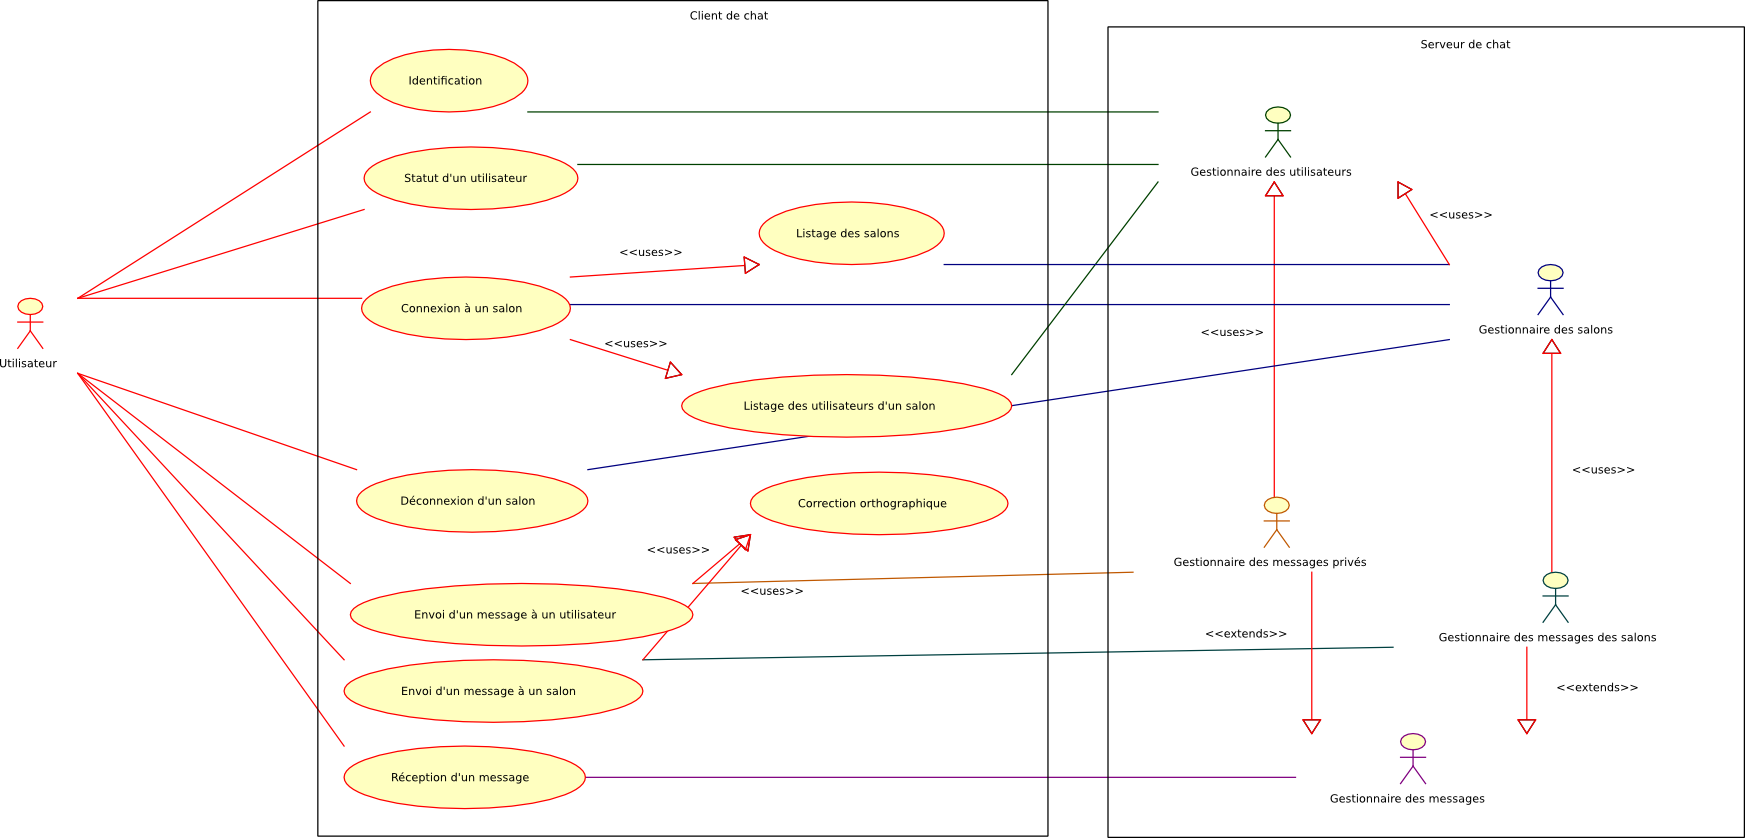
\includegraphics[angle=90,width=0.9\linewidth]{use_case.png}

\section{Diagramme de structure statique}

    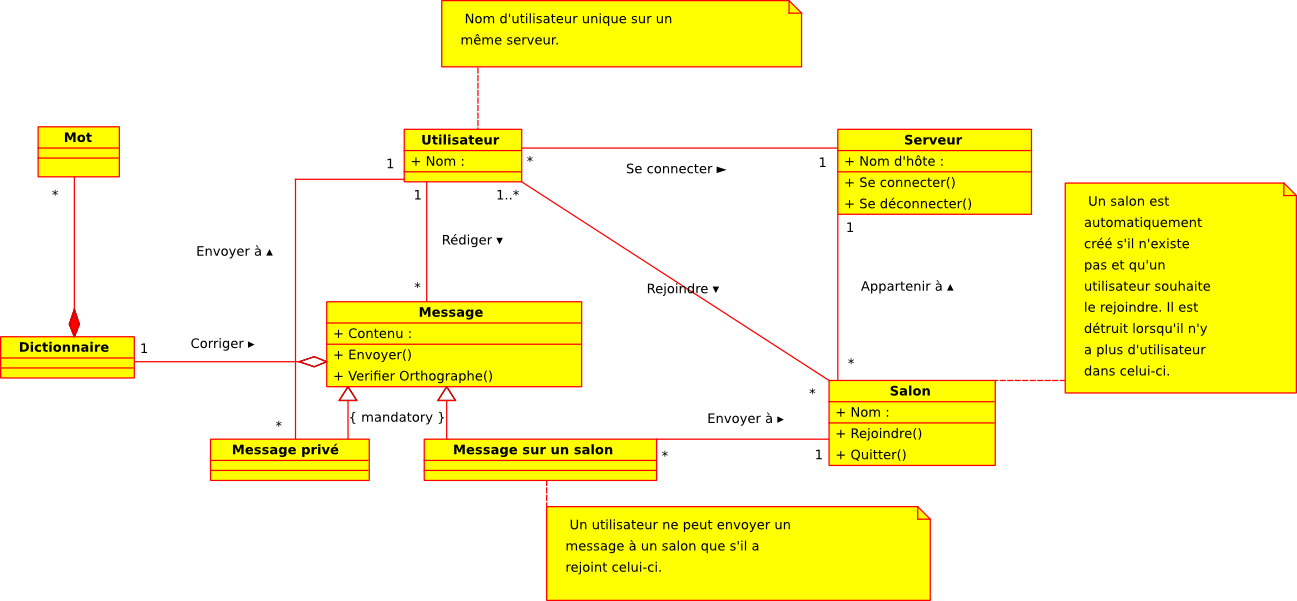
\includegraphics[angle=90,width=0.9\linewidth]{structure_statique.png}

\section{Diagramme à états}

    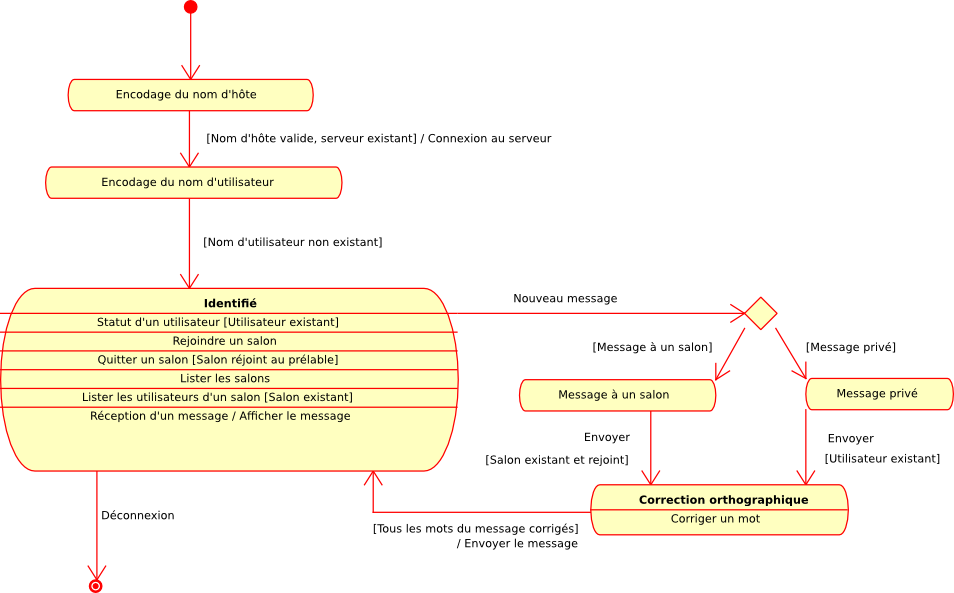
\includegraphics[angle=90,width=0.9\linewidth]{state.png}

\section{Documentation de la partie serveur}

 \subsection{Diagramme de classes du logiciel serveur}

    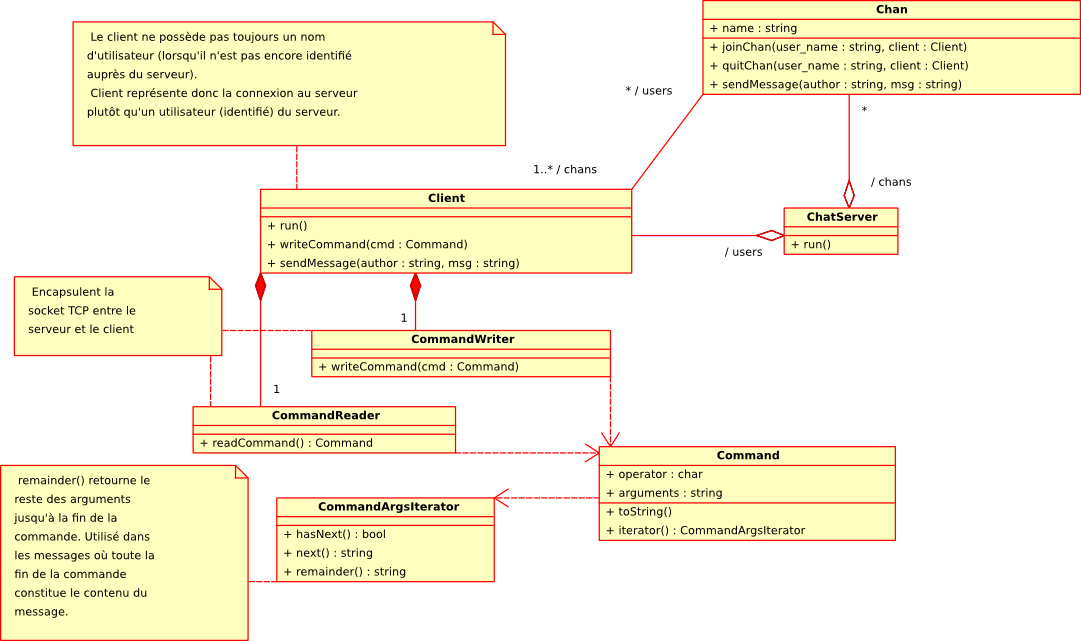
\includegraphics[angle=90,width=0.9\linewidth]{class.png}

 \subsection{Interaction typique entre un client et le serveur}

    \paragraph{}Représente une interaction typique entre le logiciel client et
les classes \textit{ChatServer}, \textit{Client} et \textit{Chan} du logiciel
serveur.

    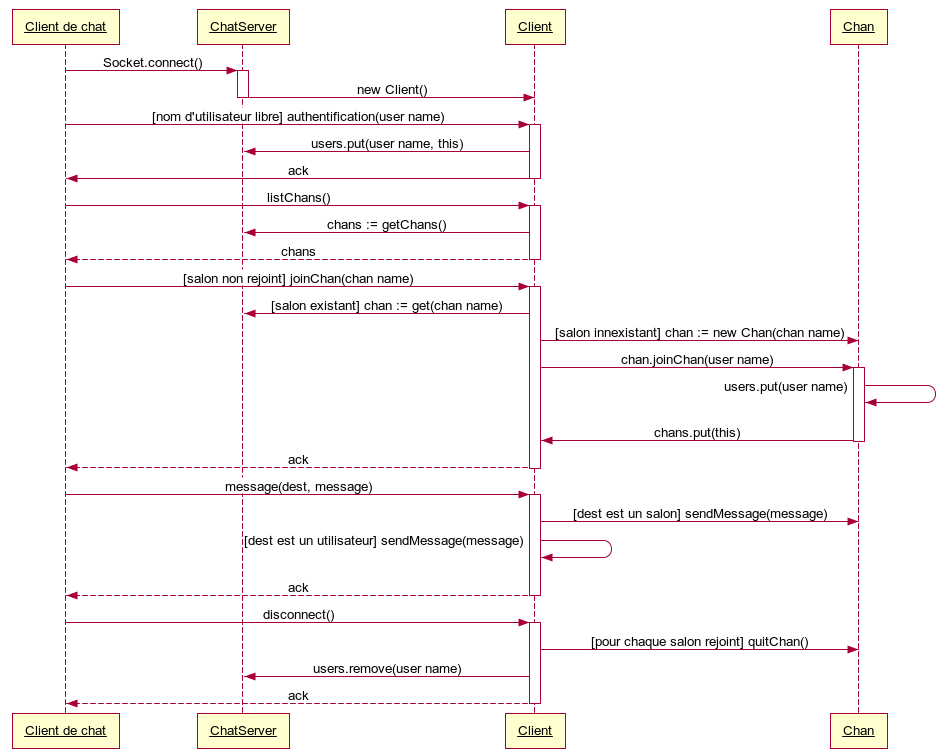
\includegraphics[angle=90,width=1\linewidth]{sequence.png}

\end{document}